\section{Vægtede grafer}

Flere problemstillinger kan modelleres ved brug af grafer med vægte tildelt kanterne. 
Det kan f.eks. være distance, den samlede rejsetid eller billetprisen for at rejse mellem to byer. 
Grafer, der har vægte tildelt kanterne, kaldes vægtede grafer. 

Der opstår jævnligt forskellige typer af problemer, der involverer vægtede grafer, hvor en kortest mulig rute, mellem to knuder i et netværk, skal bestemmes. 
Længden af en vej i en graf uden vægte er tidligere betegnet ved antallet af kanter, vejen går igennem.
I en vægtet graf er længden af vejen summen af alle kanternes vægte, der indgår i vejen.

\begin{defn}
	Lad $G = (V,E)$ være en vægtet graf. Da betegnes $d(v_i, v_j)$ som \textit{vægten} af kanten mellem to knuder $v_i, v_j \in V$.
	Så samme vis betegnes $d(e)$ som vægten af en kant $e \in E$, og $d(S)$ den summen af alle vægte i en graf $S \subseteq G$.
	Desuden er $d(e) \in \mathbb{R}_{\geq 0}$, for alle $e \in E$.
\end{defn}

\begin{exmp}
I Figur \ref{fig:weighted_graph} ses et eksempel på en vægtet graf. Den kortest mulige vej fra $A$ til $D$ må være $\lbrace A,C \rbrace$, $\lbrace C,E \rbrace$, $\lbrace E,F \rbrace$, $\lbrace F,D \rbrace$. Denne vej har en længde på $5+5+5+5=20$. 
\end{exmp}

\begin{figure}[h!]
	\centering
	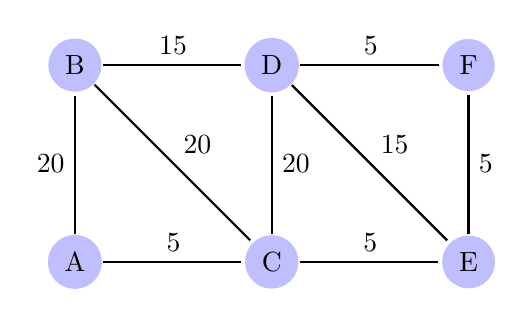
\begin{tikzpicture}[shorten >=1pt,auto,node distance=2.5cm,thick,main node/.style={circle,fill=blue!25}]                      
  \node[main node] (F) {F};                
  \node[main node] (D) [left of=F] {D};    
  \node[main node] (E) [below of=F] {E};   
  \node[main node] (B) [left of=D] {B};    
  \node[main node] (C) [below of=D] {C};   
  \node[main node] (A) [below of=B] {A};   
              
	\path[-, draw, thick]
  (A) edge node {$20$} (B)
	(B) edge node {$20$} (C)
	(B) edge node {$15$} (D)
	(C) edge node[right] {$20$} (D)
	(C) edge node {$5$} (E)
	(D) edge node {$15$} (E)
	(D) edge node {$5$} (F)
	(E) edge node[right] {$5$} (F)
	(A) edge node {$5$} (C)
	;
\end{tikzpicture}

	\caption{Eksempel på en vægtet graf.} \label{fig:weighted_graph}
\end{figure}

I et interessant problem, som involverer vægtede grafer, søges en kreds af kortest mulig totallængde, der besøger hver knude i en komplet graf præcis én gang.

I Figur \ref{fig:weighted_graph} vil en kreds af kortest mulig længde være $\lbrace A,C \rbrace$, $\lbrace C,E \rbrace$, $\lbrace E,F \rbrace$, $\lbrace F,D \rbrace$, $\lbrace D,B \rbrace$, $\lbrace B,A \rbrace$.
Denne kreds har en længde på $5+5+5+5+15+20=55$.

Der er her tale om et eksempel på \emph{Traveling Salesperson Problem}, som søger dén rækkefølge, knuderne skal besøges i, som resulterer i en kreds af kortest mulig længde. 
Dette problem vil projektet undersøge nærmere i Kapitel \ref{chap:TSP}.

\subsection{Algoritme til en kortest mulig vej}
Der er flere algoritmer, som finder den korteste vej mellem to knuder i en vægtet graf.
Et eksempel på en sådan algoritme er Dijkstras algoritme.
Algoritmen bruges til at finde den korteste vej mellem knuderne $u$ og $v$ for en ikke-orienterede vægtet graf $G=(V,E)$. Desuden algoritmen kan let tilpasses til orienterede grafer.

Algoritmen bygger på en serie af gentagelser, hvor en mængde af knuder, $S$, konstrueres, ved at tilføje én knude ved hver gentagelse, $k$.
I starten indeholder $S$ blot $u$.
En knude $v_j$, der er nabo til en knude i $S$, men ikke selv er i $S$, bliver tildelt en værdi der svarer til vægten af den kortest mulige vej fra $u$ til $v_J$, der kun indeholder knuder, der allerede er i $S$.
Her betegnes den kortest mulige vej, som den vej hvis vægt er mindst mulig. 
Ved første gentagelse må $v_j$ da være nabo til $u$.
Hvis der eksisterer flere veje fra $u$ til $v_k$, bliver $v_k$ tildelt værdien der svarer til den kortest mulige vej. 

Dijkstras algoritme starter ved at tildele $u$ værdien $0$ og de andre knuder værdien $\infty$. 
Lad her værdien for en knude $v_i$ betegnes som $L(v_i)$.
Da er $L(u) = 0$ og $L(v_i)= \infty$, for alle knuder $v_i \in V$ pånær $u$.
Disse værdier angiver længden af den korteste vej fra $a$ til de givne knuder, i starten af algoritmen, altså hvor vejen kun indeholder $u$. 
Der er da endnu ikke en vej i $S$.

Til at begynde med er $S=\empty $. 
Mængden $S$ opdateres ved at tilføje en knude $v_j$, der ikke er i $S$, og har den mindst mulige værdi.
I første skridt må den knude der vælges være netop $u$, da denne knude har den mindste værdi.
Herefter opdateres værdierne af alle knuder, som ikke er i $S$, således $L(v_i)$ bliver summen af $L(v_j)$ og $d(v_j,v_i)$, hvis denne er mindre end $L(v_i)$.
Værdien $L(v_i)$ opdateres da kun hvis der eksisterer en kant mellem $v_j$ og $v_i$, og hvis $L(v_i)$ ikke allerede har den mindst mulige værdi. 
Den måde, hvorpå algoritmen vælger en knude $v_j$, der føjes til $S$ ved hver gentagelse, er det optimale valg af knude, hvilket gør den til en grådig algoritme. 

Proceduren fortsætter med at tilføje knuder til mængden, indtil $v$ også er tilføjet.
Herefter tildeles $v$ den værdi, der svarer til længden af den korteste vej fra $u$ til $v$.

Dijkstras algoritme ses i Algoritme \ref{dijkstras_algorithm}.

\begin{algorithm}[!h]
	\caption{Dijkstras algoritme}
	\label{dijkstras_algorithm}
	\textbf{procedure} $Dijkstra(G:$ vægtet sammenhængende simpel graf) \\ 
	$\lbrace G$ har knuder $u=v_0, v_1, \dotsc , v_n=v$ og vægtene $d(v_i,v_j)$ hvor $d(v_i,v_j)= \infty $ hvis $ \lbrace v_i,v_j \rbrace $ ikke er en kant i $G \rbrace$ \\
	\textbf{for} $i:=1$ \textbf{til} $n$ \\
	$\-$ $\-$ $\-$ $\-$ $\-$ $\-$
	$L(v_i):= \infty$ \\
	$L(u):=0$ og $S:= \emptyset $ \\
	$\lbrace$ værdien er nu fastsat, så $L(u)$ er $0$, alle andre værdier er $\infty$, og $S$ er tom$\rbrace$ \\
	\textbf{så længe} $v \not\in S$ \\
	$\-$ $\-$ $\-$ $\-$ $\-$ $\-$
	$v_j:=$ en knude $\not\in S$ med hvor $L(v_j)$ er den mindste værdi blandt knuderne der ikke er i $S$ \\
	$\-$ $\-$ $\-$ $\-$ $\-$ $\-$
	$S:= S\cup \lbrace v_j \rbrace$ \\
	$\-$ $\-$ $\-$ $\-$ $\-$ $\-$
	\textbf{for} alle knuder $v_i \not\in S$ \\
	$\-$ $\-$ $\-$ $\-$ $\-$ $\-$
	$\-$ $\-$ $\-$ $\-$ $\-$ $\-$
	\textbf{hvis} $L(v_j)+d(v_j,v_i)<L(v_i)$ \textbf{så} $L(v_i):=L(v_j)+d(v_j,v_i)$ \\
	$\-$ $\-$ $\-$ $\-$ $\-$ $\-$
	$\lbrace$ dette tilføjer en knude til $S$ med minimal værdi og opdaterer værdien af knuderne $\not\in S$ $\rbrace$ \\
	\textbf{returnér} $L(v)$ $\lbrace L(v)=$ længden af den korteste vej fra $u$ til $v \rbrace$
\end{algorithm} 

\begin{thm}\label{dijkstras_theorem}
	Dijkstras algoritme finder længden af en kortest mulig vej mellem to knuder i en sammenhængende, simpel, ikke-orienteret, vægtet graf.
\end{thm}

\begin{proof}
	Induktionsantagelsen gælder for den $k$'te gentagelse. 
	Lad $v$ være knuden tilføjet til $S$ ved den $(k+1)$'te gentagelse, så $v$ er en knude, som ikke er et element i $S$ i slutningen af den $k$'te gentagelse med den mindste værdi (hvis der er flere knuder af samme værdi, vælges blot én af disse). \\
	Fra indkuktionsantagelsen ses det, at knuderne i $S$ før den $(k+1)$'te gentagelse er angivet med længden af den korteste vej fra $a$. 
	Så er $v$ angivet med længden af den korteste vej fra $v$ til $a$. 
	Hvis det ikke var tilfældet i slutningen af den $k$'te gentagelse, ville der være en vej kortere end $L_k(v)$, der indeholder en knude, som ikke er et element i $S$. 
	Lad $u$ være den første knude, som ikke er et element i $S$ i sådan en vej. 
	Der er en vej med en længde kortere end $L_k(v)$ fra $a$ til $u$ kun indeholdende knuder i $S$. 
	Dette modsiger valget af $v$, da $(i)$ holdes i slutningen af den $(k+1)$'te gentagelse.
	Lad $u$ være en knude, som ikke er et element i $S$ efter $k+1$ gentagelser. 
	En kortest mulig vej fra $a$ til $u$, som kun indeholder elementer i $S$, indeholder enten $v$ eller ikke. 
	Hvis den ikke indeholder $v$, er længden $L_k(u)$ ifølge induktionsantagelsen. 
	Hvis den derimod indeholder $v$, må der laves en vej fra $a$ til $v$ af kortest mulig længde, der indeholder alle elementerne i $S$ undtagen $v$, efterfulgt af kanten fra $v$ til $u$. I det tilfælde, vil længden være $L_k(v)+w(v,u)$. Dette viser, at $(ii)$ er sand, da $L_{(k+1)}(u)=\textrm{min} \lbrace L_k(u), L_k(v)+w(v,u) \rbrace$. 
\end{proof}
